\documentclass[11pt,a4paper]{article}
\usepackage[utf8]{inputenc}
\usepackage[T1]{fontenc}
\usepackage[spanish]{babel}
\usepackage[margin=2cm]{geometry}
\usepackage{lmodern}
\usepackage{graphicx}
\usepackage{array}
\usepackage{tabularx}
\usepackage{booktabs}
\usepackage{enumitem}
\usepackage[hidelinks]{hyperref}
\setlist[description]{leftmargin=0pt,itemsep=4pt}

\begin{document}

\begin{center}
  {\large\bfseries Universidad Técnica Estatal de Quevedo\par}
  {Facultad de Ciencias de la Computación -- Carrera de Software\par}
  \vspace{4pt}
  {Aplicaciones Distribuidas (ISR-701) -- Séptimo nivel, paralelo B\par}
  \vspace{12pt}
  {\Large\bfseries FORM-TL-01: Notas del taller\par}
  \vspace{4pt}
  {\large Modelado de comunicación entre procesos distribuidos\par}
  \vspace{10pt}
  Benites Pérez Dariem Alberto \quad Bueno Troya Erwin Daniel \quad Mendoza Villarroel Elian Jossue\par
  Docente: Gleiston Guerrero Ulloa, PhD\par
  11 de noviembre de 2026\par
\end{center}

\section{Escenario y procesos}

El escenario que nos tocó es un sistema de reservas de vuelos. Usamos los cuatro procesos que propone la guía:

\begin{description}
  \item[P1, Cliente.] La app donde el usuario busca vuelos y reserva. Solo hace de cliente.
  \item[P2, Servidor de aplicación.] El servicio de reservas. Es servidor para el cliente y, al mismo tiempo, cliente del servicio de pagos y de la base de datos.
  \item[P3, Servicio de pagos.] Cobra con un token de la tarjeta. Atiende llamadas gRPC.
  \item[P4, Base de datos.] PostgreSQL, guarda vuelos, asientos y reservas.
\end{description}

El modelo es cliente-servidor en capas: el cliente nunca habla directo con pagos ni con la base de datos, todo pasa por P2. Para PE-U1 el cliente y el servidor de aplicación se programarán en Python con sockets, y el servicio de pagos con gRPC (\texttt{grpcio}), como indica el material de la semana 3.

\section{Diagrama de comunicación}

El archivo editable está en \texttt{diagrama/diagrama-comunicacion.drawio}. Las flechas continuas son síncronas y las discontinuas, asíncronas. El orden de una reserva es 3, 4, 5, 6 y la respuesta de la 3.

\begin{figure}[h]
  \centering
  \IfFileExists{../diagrama/diagrama-comunicacion.pdf}
    {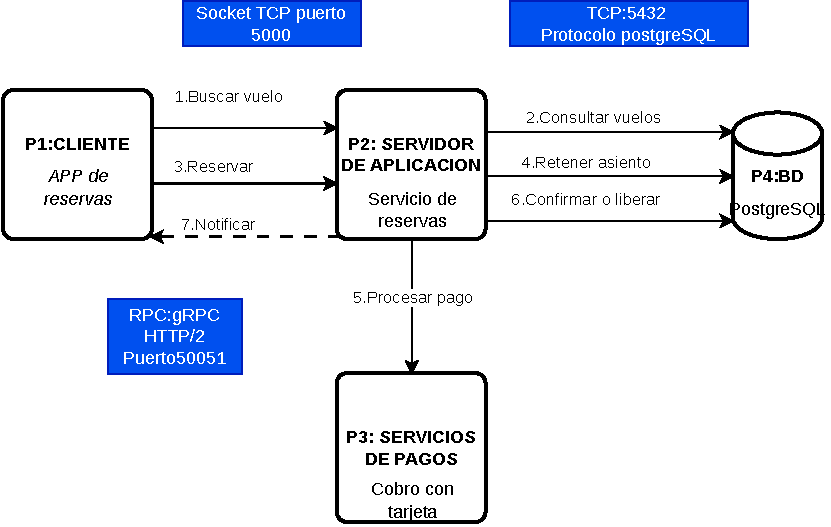
\includegraphics[width=\textwidth,height=0.75\textheight,keepaspectratio]{../diagrama/diagrama-comunicacion.pdf}}
    {\IfFileExists{../diagrama/diagrama-comunicacion.png}
      {\includegraphics[width=\textwidth,height=0.75\textheight,keepaspectratio]{../diagrama/diagrama-comunicacion.png}}
      {\fbox{\parbox{0.9\textwidth}{\centering Falta \texttt{diagrama/diagrama-comunicacion.pdf}.}}}}
  \caption{Comunicación entre los procesos del sistema de reservas de vuelos.}
\end{figure}

\section{Interacciones}

\IfFileExists{interacciones.tex}{\subsection{Resumen de las interacciones}

\begin{center}
\footnotesize
\setlength{\tabcolsep}{4pt}
\renewcommand{\arraystretch}{1.3}
\begin{tabularx}{\textwidth}{@{}c l >{\raggedright\arraybackslash}X >{\raggedright\arraybackslash}p{1.9cm} >{\raggedright\arraybackslash}p{1.6cm} >{\raggedright\arraybackslash}p{2.5cm} >{\raggedright\arraybackslash}p{2.2cm}@{}}
\toprule
\textbf{N.º} & \textbf{De $\to$ A} & \textbf{Mensaje (petición / respuesta)} & \textbf{Mecanismo} & \textbf{Tipo} & \textbf{Protocolo} & \textbf{Middleware} \\
\midrule
1 & P1 $\to$ P2 & \texttt{BUSCAR\_VUELOS}(origen, destino, fecha) / lista de vuelos & Sockets & Síncrona & TCP, puerto 5000 & Ninguno (socket de Python, JSON) \\
2 & P2 $\to$ P4 & Consulta de vuelos y asientos libres / filas encontradas & Sockets (driver de BD) & Síncrona & TCP, puerto 5432, protocolo de PostgreSQL & psycopg \\
3 & P1 $\to$ P2 & \texttt{RESERVAR}(vuelo, asiento, pasajero, id\_solicitud) / código de reserva o rechazo & Sockets & Síncrona & TCP, puerto 5000 & Ninguno (socket de Python, JSON) \\
4 & P2 $\to$ P4 & Transacción: bloquear el asiento y guardar la reserva como PENDIENTE (10 min) / OK & Sockets (driver de BD) & Síncrona & TCP, puerto 5432, protocolo de PostgreSQL & psycopg \\
5 & P2 $\to$ P3 & \texttt{ProcesarPago}(reserva, monto, token, clave) / APROBADO o RECHAZADO & RPC & Síncrona, deadline de 3 s & HTTP/2 sobre TCP, puerto 50051 & gRPC y Protocol Buffers \\
6 & P2 $\to$ P4 & Cambiar la reserva a CONFIRMADA o CANCELADA / OK & Sockets (driver de BD) & Síncrona & TCP, puerto 5432, protocolo de PostgreSQL & psycopg \\
7 & P2 $\to$ P1 & \texttt{NOTIFICAR}(cambio de vuelo o reserva vencida) / sin respuesta & Sockets & Asíncrona & TCP, puerto 5000 & Ninguno (socket de Python, JSON) \\
\bottomrule
\end{tabularx}
\end{center}

Las interacciones 1, 3 y 7 usan sockets y la 5 usa RPC con gRPC, que son los dos mecanismos que vamos a programar y comparar en PE-U1.

\subsection{Justificación de cada interacción}

\begin{description}
  \item[1. Buscar vuelos.] El cliente abre una conexión TCP con el servidor y la deja abierta mientras usa la app. Elegimos sockets porque con la conexión ya abierta cada búsqueda no tiene que volver a conectarse, y así la respuesta llega más rápido. Es síncrona porque el usuario no puede seguir hasta ver los vuelos. Los mensajes son pequeños (un JSON por línea), así que aunque haya muchas búsquedas el volumen no es un problema. TCP asegura que el mensaje llegue completo y en orden.

  \item[2. Consultar vuelos.] El servidor le pide a PostgreSQL los vuelos y los asientos libres. Por debajo también es un socket TCP, pero no lo programamos nosotros: lo maneja el driver psycopg con el protocolo propio de PostgreSQL. Es síncrona porque el servidor necesita esos datos para contestar la interacción 1.

  \item[3. Reservar.] Va por la misma conexión que la búsqueda. Es síncrona porque el usuario espera saber si su reserva quedó o no. Cada solicitud lleva un \texttt{id\_solicitud}: si la conexión se corta y el cliente vuelve a enviar lo mismo, el servidor reconoce el id y no crea una segunda reserva.

  \item[4. Retener el asiento.] Aquí lo que más importa es la consistencia: si dos personas piden el mismo asiento al mismo tiempo, solo una lo puede obtener. Por eso el servidor bloquea la fila del asiento dentro de una transacción y guarda la reserva como PENDIENTE por 10 minutos. La transacción se cierra enseguida, antes de cobrar, para que el asiento no quede bloqueado mientras se espera al servicio de pagos.

  \item[5. Procesar el pago.] Es la interacción con RPC. Usamos gRPC porque es una comunicación interna entre dos servicios del sistema: el archivo \texttt{.proto} define exactamente qué datos se envían y qué se recibe, Protocol Buffers manda los datos en binario y HTTP/2 reutiliza la conexión, por eso la latencia es baja. Es síncrona porque sin el resultado del pago no se puede confirmar la reserva. Le ponemos un deadline de 3 segundos para que el servidor no se quede esperando si pagos no contesta, y una clave de idempotencia para poder reintentar una vez sin cobrar dos veces. Al servicio de pagos solo le llega un token de la tarjeta, nunca el número.

  \item[6. Confirmar o liberar.] Con la respuesta de pagos, el servidor cambia la reserva a CONFIRMADA, o a CANCELADA y libera el asiento. Así lo que queda guardado en la base de datos coincide con lo que pasó con el pago. Recién ahí el servidor contesta al cliente la interacción 3.

  \item[7. Notificar.] El servidor avisa al cliente cuando cambia algo de su vuelo, como un retraso o un cambio de puerta, o cuando vence una reserva pendiente. Es asíncrona: el servidor manda el aviso por la conexión abierta y sigue trabajando sin esperar respuesta. Si el cliente está desconectado el aviso se pierde, pero no es grave porque al volver a conectarse consulta el estado de su reserva. Si estos avisos fueran críticos usaríamos una cola de mensajes como RabbitMQ, que guarda el mensaje hasta que se entregue.
\end{description}
}{Falta el archivo \texttt{notas/interacciones.tex}.}

\section{Exposición: preguntas y respuestas}

El ingeniero envió el taller para trabajar en casa. Hasta la fecha de esta entrega no hemos expuesto el diagrama, así que todavía no hay preguntas de otros equipos. Si se programa la exposición, aquí se agregarán las preguntas que recibamos y lo que respondimos.

\subsection{Preguntas críticas que preparamos}

Para revisar el diseño nos hicimos estas preguntas antes de exponer:

\begin{description}[style=nextline]
  \item[¿Qué pasa con la reserva si el servicio de pagos no responde?] El servidor espera como máximo 3 segundos (deadline de gRPC) y reintenta una vez con la misma clave de idempotencia, así que pagos no cobra dos veces. Si tampoco responde, la reserva se queda en PENDIENTE, el cliente recibe ``pago no confirmado'' y el asiento se libera solo cuando pasan los 10 minutos.

  \item[¿Qué pasa si dos clientes reservan el mismo asiento al mismo tiempo?] La interacción 4 bloquea la fila del asiento dentro de una transacción. El primero que llega se queda con el asiento y el segundo recibe ``asiento no disponible''. Aquí preferimos consistencia antes que disponibilidad.

  \item[¿Y si se cae el servidor después de cobrar, pero antes de confirmar?] La reserva queda en PENDIENTE con su clave de pago. Al reiniciar, el servidor revisa las reservas pendientes y le pregunta a pagos por esa clave: si el cobro existe confirma la reserva, y si no, la cancela.

  \item[¿Por qué sockets entre el cliente y el servidor y no una API REST?] La guía pide una interacción con sockets y es lo que vamos a programar en PE-U1. Con la conexión abierta, el servidor puede mandar avisos sin que el cliente pregunte (interacción 7). La desventaja es que nosotros definimos el formato de los mensajes y manejamos las reconexiones.

  \item[¿Por qué el pago es síncrono y no va por una cola de mensajes?] Porque el usuario espera la confirmación en ese momento. Con una cola habría que agregar otro proceso, el broker, y avisar del resultado después. Eso conviene si el pago tarda mucho, como una transferencia bancaria, pero no para un cobro con tarjeta.
\end{description}

\section{Declaración de uso de inteligencia artificial}

\noindent
\begin{tabularx}{\textwidth}{>{\bfseries}l >{\raggedright\arraybackslash}X}
  Herramienta: & Claude (Anthropic), modelo Claude Opus 5.5, en la aplicación Claude Code. \\
  Para qué se usó: & Para encontrar el diseño de la comunicación: qué mecanismo, protocolo y middleware usa cada interacción y por qué. Hizo un diagrama de referencia que redibujamos en draw.io, ayudo a corregir la tabla de interacciones, las justificaciones y las preguntas preparadas de estas notas. \\[4pt]
  Cómo se verificó: & Comparamos cada decisión con el material de la semana 3 (sockets, RPC, middleware y la tabla de sockets TCP frente a gRPC) y con la guía del taller: al menos cuatro procesos, una interacción con sockets y otra con RPC.
\end{tabularx}

\end{document}
